\documentclass[10pt]{article}
\usepackage{icmlko}

\icmlmeta{IP 파운데이션 월드모델}{201}{최근 가중이 이미 고르고 있었다}{두 이득을 합치러 갔다. 수동 틀에서는 거의 가법인데 등록 틀에서는 통째로 겹친다 --- 그리고 겹치는 자리를 정확히 짚을 수 있다}

\begin{document}

\twocolumn[
\icmlheader

\begin{abstract}
노트 194의 최근 가중($+$0.030)과 노트 197의 도메인별 풀링 선택($+$0.013)을
합쳤다. 순차로 --- 노트 195가 ``같이 고르면 나빠진다''를 쟀으므로. \textbf{두
답이 나온다.} 내가 손으로 만든 일곱 도메인 틀에서는 \textbf{거의 가법}이다
--- 각각 $+$0.0200 · $+$0.0133 이고 합쳐서 $+$0.0319 로 단순 합($+$0.0333)의
96\%다. 그런데 정식화로 등록해 열 도메인 전부를 쓰면 \textbf{통째로
겹친다}: 기본 $+$0.3709 $\to$ 알파 20 으로 $+$0.3744 $\to$ 최근 가중으로
$+$0.4036 $\to$ \textbf{도메인 선택을 더해도 $+$0.4043}($+$0.0007 ·
$t{=}0.13$). 선택 \emph{단독}은 $+$0.0160 인데 최근 가중 위에서는 0 이다.
\textbf{겹치는 자리를 짚을 수 있다} --- 모바일의 안쪽 격차가 가중 없이
$+$0.143 인데 $\tau{=}2$ 에서 \textbf{$+$0.004} 로 사라진다. 최근 가중이
옛 행을 덜 믿게 만들자 풀링 모형이 모바일에게 자기 모형만큼 잘 맞게 된
것이다. \textbf{선택이 하던 일을 가중이 이미 하고 있었다.} 이 흐름에서
``모형이 이미 쓰고 있는 것을 명시로 세우면 잉여다''의 \textbf{네 번째}
사례다(노트 175의 문서 존재 축 $+$0.0000, 노트 181의 속편 축 $+$0.0022,
노트 188의 무리 쌓기, 그리고 이것). 곁가지로 구현 가드 하나를 얻었다 ---
처음 등록한 \texttt{F21} 이 $+$0.3780 으로 오히려 나빴는데, \textbf{팝업처럼
학습이 열여섯 행뿐인 도메인에도 혼자 모형을 세우고 있었다.} 최소 150행
조건을 넣으니 $+$0.4043 이 된다. \textbf{$+$0.026 이 그 한 줄에 있었다.}
등록 형태 중 선형 최고는 이제 \texttt{F21\_recentpick} 의 $+$0.4043 이고
챔피언 \texttt{F18\_bagboost}($+$0.4490)와의 격차가 0.078 에서
\textbf{0.045} 로 줄었다.
\end{abstract}
]

\begin{figure*}[t]
\centering
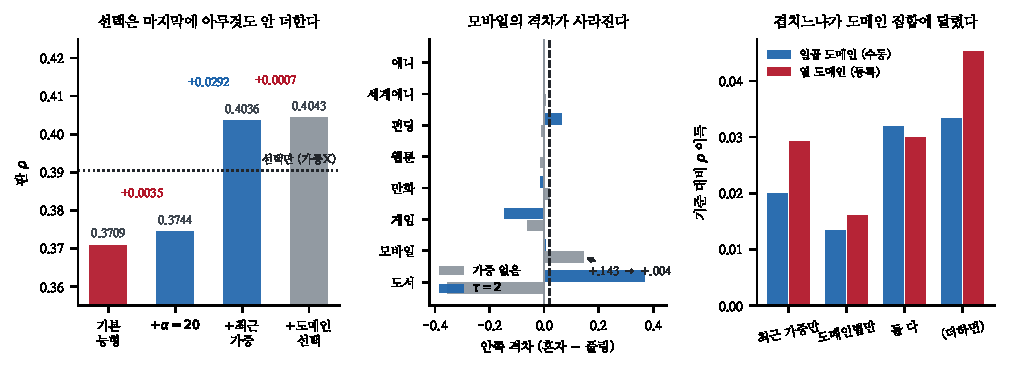
\includegraphics[width=\textwidth]{figs/already.pdf}
\caption{왼쪽 --- 선택은 마지막에 아무것도 안 더한다. 가운데 --- 모바일의
격차가 사라진다. 오른쪽 --- 겹치느냐가 도메인 집합에 달렸다.}
\end{figure*}

\section{사다리}

\begin{table}[t]
\centering\tsize
\caption{열 도메인 등록 틀. 하나씩 얹는다.}
\begin{tabular}{lrr}
\toprule
& 판 $\rho$ & 더한 값 \\
\midrule
① 기본 능형 ($\alpha{=}1$) & .3709 & \\
② $+\alpha{=}20$ & .3744 & $+$.0035 \\
\textbf{③ $+$최근 가중} & \textbf{.4036} & \textbf{$+$.0292} \\
\textbf{④ $+$도메인 선택} & \textbf{.4043} & \textbf{$+$.0007} \\
\midrule
⑤ 선택만 (가중 없이) & .3904 & $+$.0160 \\
\bottomrule
\end{tabular}
\end{table}

\claimx{\textbf{선택 단독은 $+$0.0160 인데 가중 위에서는 $+$0.0007
이다}($t{=}0.13$). 두 손잡이가 같은 것을 잡고 있다.}{①$\to$④ 전체는
$+$0.0334($t{=}5.13$)로 확실하다 --- \textbf{이득은 진짜인데 그 안에서
선택 몫이 없다.}}

\section{겹치는 자리}

\begin{table}[t]
\centering\tsize
\caption{안쪽 격차(혼자 $-$ 풀링). 문턱 0.02.}
\begin{tabular}{lrrr}
\toprule
& 가중 없음 & $\tau{=}2$ & 변화 \\
\midrule
\textbf{모바일} & \textbf{$+$.143} & \textbf{$+$.004} & \textbf{$-$.139} \\
도서 & $-$.352 & $+$.367 & $+$.719 \\
게임 & $-$.061 & $-$.146 & $-$.084 \\
만화 & $+$.020 & $-$.012 & $-$.032 \\
웹툰 & $-$.012 & $+$.002 & $+$.015 \\
세계애니 & $+$.004 & $-$.000 & $-$.004 \\
애니 & $-$.001 & $-$.000 & $+$.000 \\
\bottomrule
\end{tabular}
\end{table}

\claimx{\textbf{모바일의 격차가 사라진다}($+$0.143 $\to$ $+$0.004). 노트
197에서 이 이득의 93\%가 모바일 하나였으니, 그 하나가 사라지면 선택이 할
일이 없다.}{읽기가 자연스럽다 --- 최근 가중이 옛 행을 덜 믿게 만들자
\textbf{풀링 모형이 모바일에게 자기 모형만큼 잘 맞는다.} 모바일이 풀에서
빠지고 싶었던 까닭은 남의 \emph{옛} 자료 때문이었다.}

\claimx{\textbf{도서는 반대로 요동친다}($-$0.352 $\to$ $+$0.367). 학습이
80행이라 되뽑기 하나에 부호가 뒤집힌다 --- \textbf{작은 도메인의 격차는
못 믿는다.}}{그래서 최소 행 조건이 필요했다(다음 절).}

\section{두 틀이 다른 답을 준다}

\begin{table}[t]
\centering\tsize
\caption{같은 두 손잡이, 다른 도메인 집합.}
\begin{tabular}{lrr}
\toprule
& 일곱 (수동) & 열 (등록) \\
\midrule
최근 가중만 & $+$.0200 & $+$.0292 \\
도메인 선택만 & $+$.0133 & $+$.0160 \\
\textbf{둘 다} & \textbf{$+$.0319} & \textbf{$+$.0299} \\
(더하면) & $+$.0333 & $+$.0452 \\
\midrule
겹침 & 4\% & \textbf{34\%} \\
\bottomrule
\end{tabular}
\end{table}

\claimx{\textbf{일곱 도메인 틀에서는 96\% 가법이고 열 도메인 틀에서는 66\%
다.} 같은 두 손잡이인데 도메인 집합이 답을 바꾼다.}{일곱 틀은 팝업 · 만화 ·
아이돌을 아예 뺐다(학습 60행 · 유보 20행 조건). 그 셋이 들어오면 풀링
모형이 달라지고 각 도메인의 격차도 달라진다 --- \textbf{풀은 부분합이
아니다.}}

\section{구현 가드 하나}

\claimx{\textbf{처음 등록한 F21 이 $+$0.3780 으로 오히려 나빴다.} 팝업은
학습이 열여섯 행인데(노트 132) 거기에 혼자 모형을 세우고, 안쪽 격차에서
우연히 이기면 그 도메인 예측이 통째로 잡음이 된다.}{최소 150행 조건을
넣으니 $+$0.4043 이다 --- \textbf{$+$0.026 이 그 한 줄에 있었다.} 노트
183의 그늘 가드가 잡을 종류인데, 이건 한 정식화 \emph{안}에서 일어나므로
가드가 못 본다.}

\section{네 번째 잉여}

\begin{table}[t]
\centering\tsize
\caption{모형이 이미 쓰고 있는 것을 명시로 세운 사례.}
\begin{tabular}{lrl}
\toprule
& 더한 값 & \\
\midrule
노트 175 문서 존재 축 & $+$.0000 & $t{=}0.0$ \\
노트 181 속편 축 & $+$.0022 & $t{=}0.95$ \\
노트 188 무리 쌓기 & $-$.0732 & 오히려 해 \\
\textbf{노트 201 도메인 선택} & \textbf{$+$.0007} & $t{=}0.13$ \\
\bottomrule
\end{tabular}
\end{table}

\claimx{\textbf{네 번째다.} 앞의 셋은 ``자질''이었고 이번엔 ``얼개''인데
같은 모양이다 --- 이미 흐르고 있는 정보를 다시 명시하면 잉여
다.}{\textbf{다만 이번엔 순서가 있다} --- 선택을 먼저 하고 가중을 나중에
했으면 반대로 보였을 것이다. 노트 195가 ``순차로 하라''고 했는데
\textbf{순서 자체는 안 정했다.}}

\begin{table}[t]
\centering\tsize
\caption{지금 포트폴리오.}
\begin{tabular}{lr}
\toprule
F18 배깅 (챔피언) & .4490 \\
F8 부스트 & .4404 \\
\textbf{F21 최근·선택} & \textbf{.4043} \\
F6 능형 최근 & .4004 \\
F10 도메인별 & .3914 \\
F6 능형 & .3709 \\
\bottomrule
\end{tabular}
\end{table}

\begin{table}[t]
\centering\tsize
\caption{남은 것.}
\begin{tabular}{ll}
\toprule
\textbf{순서} & 선택 먼저 · 가중 나중이면 어떻게 되나 \\
최소 행 & 150 은 손으로 정한 값 \\
\textbf{트리} & 최근 가중을 F18 에 --- 규약이 막고 있다 \\
\bottomrule
\end{tabular}
\end{table}

첫 줄이 곧바로 잴 수 있고 이 노트의 결론을 시험한다. ``선택이 잉여''라는
결론은 \emph{가중을 먼저 건} 순서에서 나왔다. 순서를 뒤집어 선택을 먼저
하고 그 위에 가중을 얹으면 \textbf{가중이 잉여로 보일 수도 있다} --- 그러면
두 손잡이가 대등하게 겹치는 것이고, 아니면 정말로 가중이 더 근본이다.
\textbf{순서를 바꿔 재는 것이 이 노트를 반증하거나 굳힌다.}

\end{document}
